\documentclass[12pt,letterpaper]{article}
\usepackage{pdfpages}
\usepackage{fancyhdr}
\usepackage[colorlinks=true, urlcolor=blue, linkcolor=blue]{hyperref}
\usepackage{graphicx}
\usepackage[top=1.4in, left=0.5in, right=0.5in, bottom=0.8in]{geometry}
\usepackage[T1]{fontenc}
\usepackage{helvet}
\pagestyle{fancy}
\renewcommand{\headrulewidth}{0pt}
\renewcommand{\footrulewidth}{0pt}
\setlength{\parindent}{0em}
\setlength{\parskip}{1em}


\fancyfoot[C]{\setlength{\unitlength}{1in}\begin{picture}(5,0)\put(-1.8,-1){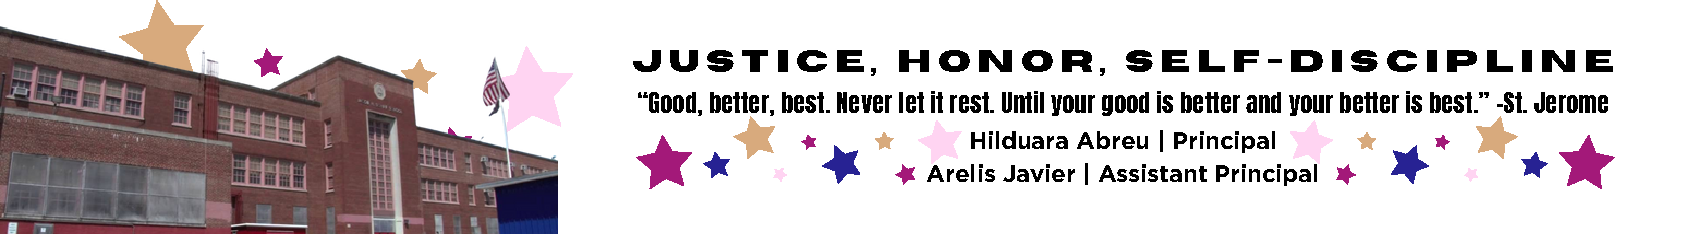
\includegraphics[width=8.8in,height=1.3in]{logo-1}}\end{picture}}
\fancyhead[C]{\setlength{\unitlength}{1in}\begin{picture}(5,0)\put(-1.9,-1){
\includegraphics[width=8.9in,height=1.3in]{logo-2}}\end{picture}}

\pagenumbering{gobble}
\addtolength{\evensidemargin}{-2in}
\addtolength{\topmargin}{-0.5in}
\addtolength{\textwidth}{0in}
%%%%%%%%%%%%%%%%%%%%%%%%%%%%%%%%%%%%%%%%%%%%%%%%%%%%%%%%%%%%%%%%%%

\begin{document}
\vspace*{0.5in}
Date: \href{https://www.ps192.org/apps/bbmessages/show_bbm.jsp?REC_ID=139439}{September 14, 2023} 

\textbf{Subject: Use of Electronic Devices School Policy}

\textbf{Use of Electronic Devices:}

Although it is not recommended, students are permitted to bring the following
electronic items to school: cell phones; and/or portable music and entertainment
systems, such as i Pods, and MP3 players. The student and/ or parent is 
responsible for the safety and security of the device and must be aware that
facilities are not available to charge said devices in school.

\textbf{Permitted Use of Electronic Devices:}

Cell phones, computing devices, and portable music and entertainment systems may be used: Before 8:00 am or after 3:35 pm anywhere in the building where it will 
not serve as a distraction to educational activities, including teams, clubs, or
other school sanctioned programs.

\textbf{Prohibited Use of Electronic Devices:}

Cell phones, computing devices, and portable music and entertainment systems may not:
\begin{itemize}
\item Be turned on or used during instructional time, except for instructional and educational purposes with the explicit approval of the teacher; and/or 
\item Be turned on or used during the administration of any school quiz, test or
examination, except where such use has been explicitly authorized by the school 
or is contained in an Individualized Education Program or Section 504
Accommodation Plan; and/or 
\item Be in the possession of students (including on their person or in a bag)
during the school’s bell schedule; and/or 
\item Be turned on or used during school fire drills or other emergency
preparedness exercises; and/or
\item Be used in bathrooms; and/or 
\item Be used during lunch in the cafeteria and/or schoolyard; and/or 
\item Be used between classes when in the hallways and stairwells; and/or 
\pagebreak
\vspace*{2cm}
\item Be used in violation of any provision of the DOE’s Discipline Code, the 
school’s policy, Chancellor’s Regulation A-413, and/or the DOE’s Internet 
Acceptable Use and Safety Policy (“IAUSP”)
\end{itemize}
\textbf{Violations for Use of Electronic Devices:}

Violations of this policy will be subject to disciplinary action, which may include:
\begin{itemize}
\item Device Confiscation - Confiscated items will only be returned to the 
parent/legal guardian following a behavioral conference regarding the violation 
of the school discipline code;and/or
\item Privilege Revocation – Students may lose the privilege to bring electronic
items to school; and/or
\item Additional Disciplinary Measure - in accordance with the guidance 
interventions and disciplinary responses set forth in the DOE Discipline Code.
\end{itemize}

Warmest regards,


\includegraphics[width=0.2\textwidth]{hil_signature}

\textbf{Principal P.S. 192}

\textit{The School of Joyful Learning!}

\url{www.ps192.org}

\end{document}

\end{document}
